\section{Méthodologie proposée}

\subsection{Description du jeu de données}
\paragraph{Source et variables.} Nous utilisons le fichier fourni avec le sujet (\texttt{Depression Oxidative Stress Mitochondrial.csv}) : 2\,621 lignes, 15 colonnes, aucune valeur manquante. Il compte autant d'observations que les données brutes de la cohorte de l'article source (2\,621 observations recueillies de 2002 à 2015) ; il semble donc correspondre à l'état \emph{antérieur} au filtrage sur la dernière visite de chaque patient, qui avait ramené l'effectif à 830 \cite{bader2024}. Les biomarqueurs ne sont toutefois pas ceux de l'article : le fichier contient trois dosages, nommés \texttt{Humanin}, \texttt{MOTSc} et \texttt{P66}, que nous interprétons comme deux peptides dérivés de l'ADN mitochondrial (humanine, MOTS-c \cite{lee2015}) et la protéine adaptatrice p66\textsuperscript{Shc}, régulatrice du stress oxydatif \cite{migliaccio1999} (interprétation déduite des noms de colonnes ; les unités ne sont pas documentées). Le tableau~\ref{tab:vars} résume les variables : 12 prédicteurs au lieu de 14.

\begin{table}[t]\centering\caption{Variables du jeu de données ($n=2\,621$).}\label{tab:vars}
\footnotesize
\begin{tabular}{@{}p{2.4cm}p{3.1cm}p{2.3cm}@{}}
\toprule Variable & Description & Valeurs / plage \\\midrule
Humanin, MOTSc, P66 & biomarqueurs mitochondriaux & $4{,}6$--$933$ ; $66{,}7$--$1\,808$ ; $5{,}6$--$148$ \\
ACE-Update & haplotype ACE & 1, 2, 3 (« 3+ » $\to$ 3) \\
OtherMeds-Depression & antidépresseurs & oui / non \\
Gender & sexe & F ($57$\,\%) / M \\
BirthAge & âge (années) & 25--104 \\
DM-Status, DM-MedUse & diabète, traitement & oui / non \\
CVD-Revised & maladie cardiovasculaire & oui / non \\
HT-Status, HT-MedUse & hypertension, traitement & oui / non \\\midrule
PHQ-9-Score (cible) & score du questionnaire & 0--24 \\
\bottomrule\end{tabular}
\end{table}

\paragraph{Prétraitement.} Les colonnes \texttt{Patient} (pseudonyme propre à chaque visite : 2\,621 identifiants distincts, donc inutilisable pour regrouper les visites d'un même patient) et \texttt{ScreenYear} (variable administrative) sont écartées. Les variables binaires sont codées 0/1 et l'haplotype ACE reste ordinal. La standardisation (moyenne nulle, écart-type unitaire, comme dans l'article) est placée \emph{dans} le pipeline et ajustée uniquement sur la partie d'entraînement de chaque pli. Deux cibles sont construites avec les seuils de l'article : binaire (PHQ-9\,$>4$ : 28,7\,\% de déprimés) et quatre classes (0--4, 5--13, 14--20, $\geq 21$ : 1\,869 / 648 / 73 / 31 lignes, soit 71,3 / 24,7 / 2,8 / 1,2\,\%, figure~\ref{fig:eda}) ; ces seuils diffèrent des seuils usuels du PHQ-9 (5, 10, 15, 20) \cite{kroenke2001}. La corrélation de Pearson entre biomarqueurs et PHQ-9 est très faible ($|r|\leq 0{,}06$), alors que l'âge ($-0{,}15$) et le diabète ($+0{,}29$) ressortent davantage.

\begin{figure}[t]\centering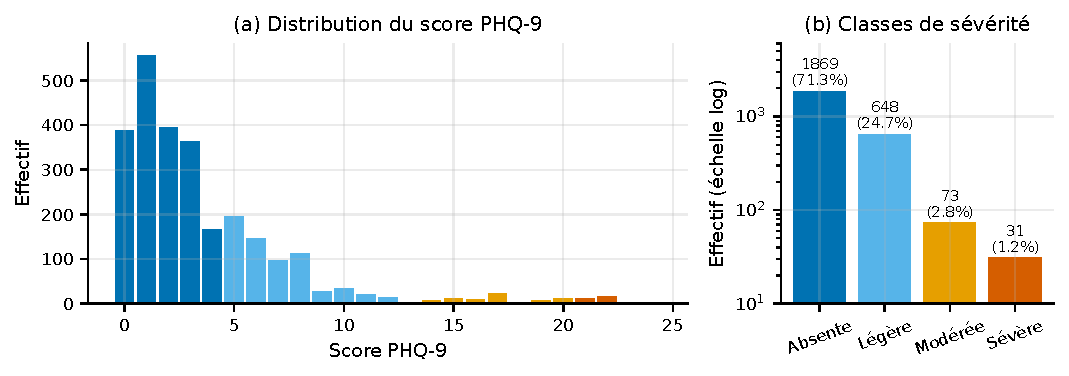
\includegraphics[width=\columnwidth]{../figures/eda_distribution.pdf}
\caption{Distribution du score PHQ-9 et des quatre classes de sévérité.}\label{fig:eda}\end{figure}

\paragraph{Audit de fuite de données.} Un Random Forest par défaut entraîné sur les \emph{trois} biomarqueurs seuls atteint une AUC de 0,94 en validation croisée aléatoire, bien au-delà du 0,84 de l'article avec cinq biomarqueurs et neuf variables, alors que les corrélations sont quasi nulles : ce résultat est suspect. Nous avons donc audité le fichier (figure~\ref{fig:leak}, tableau~\ref{tab:leak}).
\begin{itemize}[leftmargin=*,itemsep=0pt,topsep=2pt]
\item \textbf{Valeurs dupliquées.} 67\,\% (Humanin), 71\,\% (MOTSc) et 85\,\% (P66) des lignes partagent leur valeur avec au moins une autre ligne, ce qui est improbable pour des dosages à deux ou trois décimales. Le plus grand groupe de triplets identiques compte 36 lignes mêlant les deux sexes, les trois génotypes ACE et des âges de 46 à 84 ans : il ne peut s'agir d'une même personne.
\item \textbf{Lien avec la cible.} Les lignes qui partagent un triplet de biomarqueurs ont la même classe de sévérité dans 98,9\,\% des cas, contre 74,0\,\% lorsque les étiquettes sont permutées au hasard.
\item \textbf{Conséquence.} L'AUC de la RF passe de 0,94 (découpage aléatoire) à 0,89 (groupes par triplet), 0,82--0,86 (une ligne par triplet) puis à 0,60 (biomarqueurs seuls) et 0,72 (toutes variables) sur le sous-ensemble de 228 lignes dont \emph{aucune} valeur n'est partagée ; le contrôle par permutation des étiquettes donne bien 0,50 sur le jeu complet.
\end{itemize}
Ces constats sont compatibles avec une imputation par donneurs conditionnée aux classes, telle que décrite dans la méthode de Jelinek \emph{et al.} \cite{jelinek2014} citée par l'article source : les valeurs imputées « encodent » alors la cible. Nous ne pouvons toutefois pas le vérifier sans documentation du jeu de données ; c'est une \emph{hypothèse}. Il est impossible de regrouper les lignes par valeur partagée (une composante connexe unique contient 2\,148 des 2\,621 lignes), d'où deux \textbf{régimes d'analyse} :
\begin{itemize}[leftmargin=*,itemsep=0pt,topsep=2pt]
\item \textbf{complet} (2\,621 lignes) : protocole de l'article ; ses scores doivent être lus comme un plafond \emph{optimiste} ;
\item \textbf{propre} (228 lignes, dont 62 déprimées) : lignes dont les trois valeurs sont uniques dans le fichier, approximation des dosages réellement mesurés. Il ne compte que 7 cas modérés et 3 sévères : seule la tâche binaire y est étudiée. Ce choix peut introduire un biais de sélection.
\end{itemize}

\begin{figure*}[t]\centering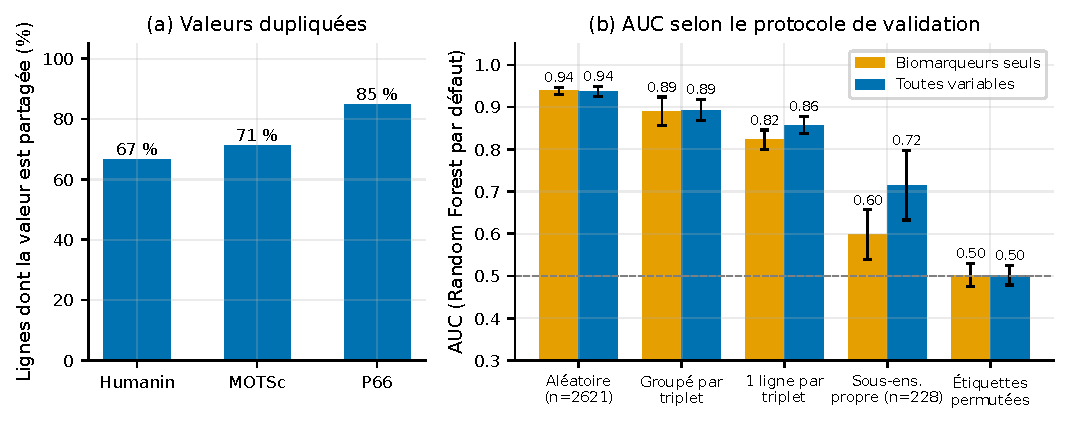
\includegraphics[width=0.82\textwidth]{../figures/leakage_audit.pdf}
\caption{Audit du fichier : (a) part des lignes dont la valeur de biomarqueur est partagée ; (b) AUC d'un Random Forest par défaut selon le protocole de validation (5 répétitions $\times$ 5 plis, barres : écart-type).}\label{fig:leak}\end{figure*}

\begin{table}[t]\centering\caption{AUC du RF par défaut (binaire) selon le protocole de validation (moyenne $\pm$ écart-type sur 25 plis).}\label{tab:leak}
\footnotesize\begin{tabular}{lcc}
\toprule
Protocole & Biomarq. seuls & Toutes var. \\
\midrule
Aléatoire ($n=2621$) & 0,938 $\pm$ 0,009 & 0,937 $\pm$ 0,012 \\
Groupé par triplet & 0,890 $\pm$ 0,034 & 0,893 $\pm$ 0,025 \\
1 ligne/triplet ($n=1571$) & 0,822 $\pm$ 0,023 & 0,858 $\pm$ 0,021 \\
Sous-ens. propre ($n=228$) & 0,598 $\pm$ 0,059 & 0,715 $\pm$ 0,083 \\
\midrule
Permutation ($n=2621$) & 0,502 $\pm$ 0,028 & 0,502 $\pm$ 0,023 \\
Permutation ($n=228$) & 0,518 $\pm$ 0,081 & 0,524 $\pm$ 0,096 \\
\bottomrule
\end{tabular}
\end{table}

\subsection{Reproduction du baseline}
La baseline reprend le protocole de \cite{bader2024} : découpage stratifié 70/30, standardisation, six classifieurs (LR, RF, KNN, SVM, NB, ANN) puis variantes pondérées (WLR, WRF avec les poids de l'éq.~\eqref{eq:weights}) et RF-SMOTE, en classification binaire et à quatre classes, avec deux jeux de variables : biomarqueurs seuls (MDP) et toutes variables (ALL). Les modèles utilisent leurs \textbf{hyperparamètres par défaut} (RF : 100 arbres ; KNN : $k=5$ ; SVM RBF : $C=1$ ; LR : $\ell_2$, $C=1$ ; ANN : une couche cachée de 100 neurones ReLU, 350 itérations, comme indiqué dans l'article), car les grilles de l'annexe de \cite{bader2024} ne figurent pas dans le texte principal. Cette reproduction porte sur le \emph{protocole} et non sur les valeurs : biomarqueurs, effectif (2\,621 contre 830) et nombre de variables (12 contre 14) diffèrent ; seule une comparaison qualitative est possible.

\subsection{Stratégie d'amélioration}
\begin{enumerate}[leftmargin=*,itemsep=0pt,topsep=2pt,label=\textbf{(\Alph*)}]
\item \textbf{Optimisation d'hyperparamètres.} Pour chaque modèle : \texttt{GridSearchCV} (grilles de l'annexe~\ref{app:grids}), \texttt{RandomizedSearchCV} (30 tirages dans des distributions, dont des lois log-uniformes pour $C$, $\gamma$, $\alpha$) et, pour la WRF, une recherche bayésienne TPE (Optuna) sur le même espace et le même budget (30 essais $\times$ 5 plis).
\item \textbf{Pondération et modèle ajouté.} WLR, WRF, RF-SMOTE comme dans l'article, plus WHGB (\emph{gradient boosting} par histogrammes pondéré), pour tester si un autre ensemble d'arbres améliore la WRF.
\item \textbf{Évaluation rigoureuse.} Validation croisée imbriquée (scores appariés avant/après), intervalles de confiance par \emph{bootstrap} sur le test, et régime « propre » de l'audit.
\item \textbf{Inférence statistique} sur les scores appariés (§\ref{sec:proto}).
\end{enumerate}

\subsection{Protocole expérimental}\label{sec:proto}
\paragraph{Séparation des données.} Un découpage 70/30 stratifié (graine 42) isole le jeu de test, utilisé une seule fois par modèle. Toutes les recherches s'exécutent sur les 70\,\% d'entraînement, par validation croisée stratifiée à 5 plis, avec pour critère l'AUC-ROC (macro un-contre-tous à quatre classes). Le meilleur modèle est ré-entraîné sur tout l'entraînement. Parmi les variantes optimisées, la méthode retenue pour les figures est celle dont l'\emph{AUC en validation croisée} est maximale : le test n'intervient jamais dans ce choix.

\paragraph{Répétitions.} Un seul découpage 70/30 produit des estimations très bruitées (le test ne contient que 9 cas sévères dans le jeu complet). Nous ajoutons donc une validation croisée \textbf{imbriquée} : boucle externe stratifiée $5\times2$ (10 scores appariés par modèle), boucle interne = \texttt{RandomizedSearchCV} à 15 candidats et 5 plis. Pour chaque pli externe, le modèle par défaut et le modèle optimisé sont évalués sur le même sous-ensemble de test.

\paragraph{Métriques et tests.} Exactitude, précision, rappel et $F_1$ (pondérés), $F_1$ macro, exactitude équilibrée, AUC-ROC et AUC-PR ; intervalles à 95\,\% par \emph{bootstrap} (1\,000 rééchantillonnages du test). Gain d'optimisation par modèle : $t$ apparié, $t$ corrigé de Nadeau--Bengio ($p_{NB}$) et Wilcoxon ($p_W$, corrigé de Holm sur les dix modèles) ; comparaison des modèles : Friedman et Conover \cite{demsar2006,terpilowski2019}.

\subsection{Implémentation}\label{sec:impl}
Python 3.13.2 ; scikit-learn 1.6.1 \cite{pedregosa2011}, imbalanced-learn 0.14.2 \cite{lemaitre2017}, Optuna 4.3.0 \cite{akiba2019}, SciPy 1.17.1 \cite{virtanen2020}, scikit-posthocs 0.18.0 \cite{terpilowski2019}, statsmodels 0.14.4, pandas 2.2.3 \cite{mckinney2010}, NumPy 2.3.5 \cite{harris2020}, matplotlib 3.10.3 \cite{hunter2007}. Toutes les graines sont fixées à 42 (découpages, modèles, recherches, Optuna). Le standardiseur et SMOTE sont ajustés \emph{à l'intérieur} de chaque pli, via un \texttt{Pipeline} (\texttt{imblearn.pipeline} pour SMOTE), afin d'éviter toute fuite supplémentaire. Le code et les versions exactes sont fournis (\texttt{requirements.txt}, \texttt{README.md}).
